%!TEX root = ../dissertation.tex

\chapter{Solution}
\label{chapter:solution}

% Smart Place Architecture
\section{Smart Place Architecture}
\label{sec:smart_place_architecture}
% TODO : Update this section
As described before, a smart place is composed by several smart objects that generate data that is
processed by the IoT application. However, to process all that data an infrastructure is required to
support the IoT application. These infrastructure is composed by RFID tags, sensors, readers and
servers, as illustrated in Figure 2. Although this infrastructure can support the IoT application
in the smart place, this architecture presents several issues regarding the deployment of the
application, the low scalability, the costs of infrastructure and its maintenance.\\

By converging the IoT applications with the Cloud computing paradigm the objective is simplify the
smart space architecture by leveraging the required infrastructure by these applications to the
Cloud providers, as illustrated in Figure 3, allowing to take advantage of the benefits offered by
Cloud computing.\\

The convergence between the IoT applications and the Cloud allow to simplify the architecture of the
smart place in a significantly way. However, as earlier mentioned these solution still presents some
issues to be resolved, namely the deployment of the application.

\subsection{Fog Configuration}
\label{sub:sol_fog}

\subsection{Cloud Configuration}
\label{sub:sol_cloud}


% Provisioning
\section{Provisioning}
\label{sec:provisioning}
Cloud4Things is a solution that automates the provisioning of software for Internet of Things applications
in the cloud. Our solution relies on configuration management tools that leverage existing software
stacks - e.g RFID software. In Figure 2 we present the architecture of Cloud4Things.\\

% C4T conceptual architecture
\begin{figure}[ht!]
  \centering
  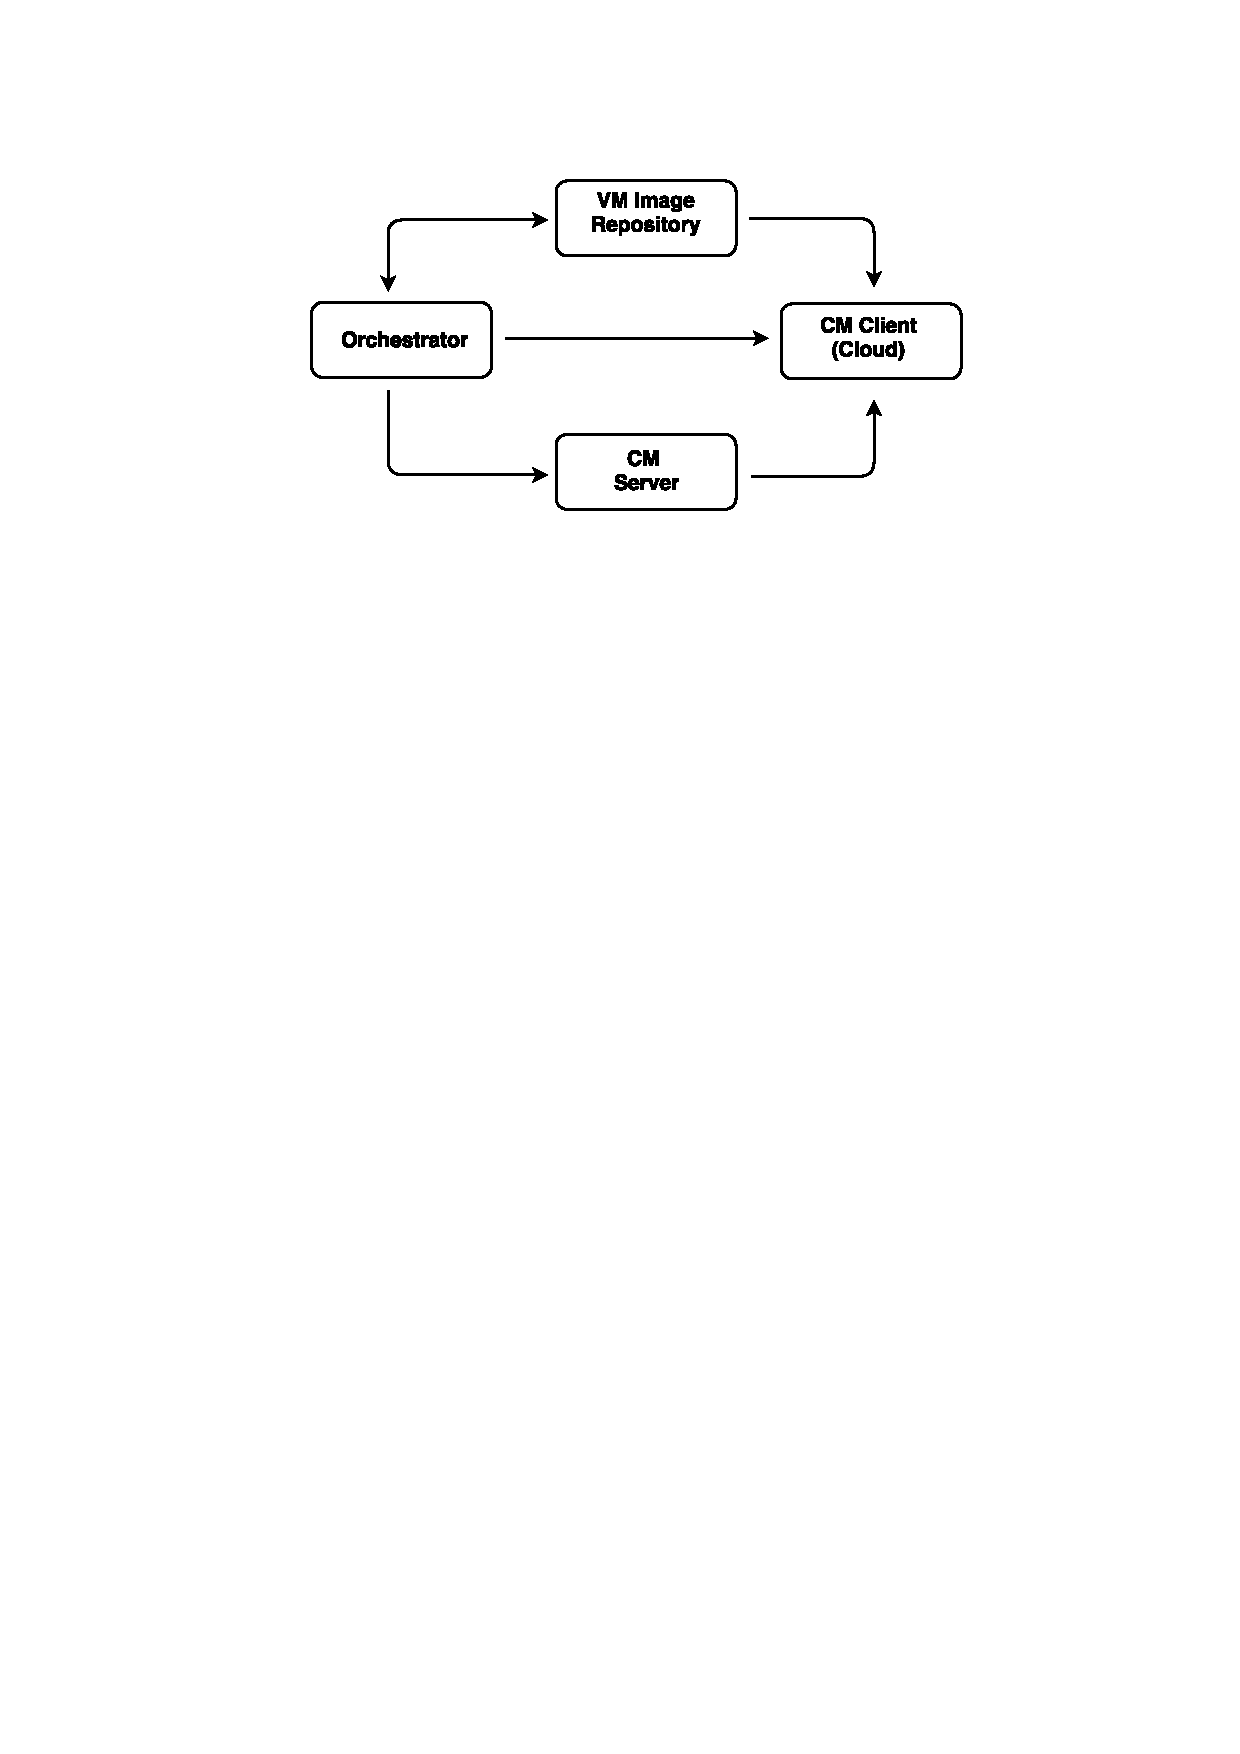
\includegraphics[width=.7\textwidth]{images/c4t-generic-solution.pdf}
  \caption{Cloud4Things conceptual architecture.}
  \label{fig:c4t_generic_solution}
\end{figure}

In our architecture, the provisioning policies and software images of a smart place are defined and
configured in a local environment and then uploaded to its respective repositories. When the provisioned
request is performed - through a configuration management interface in a local environment - the
configuration management (CM) client in the server node pulls the polices from the configuration
management server, a centralized server that is responsible to maintain a consistent state of the
provisioned nodes in the cloud. In order to enforce the polices, the CM client pulls the software
images from a central repository and then performs the provisioning and configuration of the software.
After provisioning the infrastructure the CM client periodically polls the CM server in order to
determine if its current state is consistent with the most recent policy.
